\section{Auswertung}
\subsection{Verifizierung der Funktionsweise des Lock-In-Verstärkers.}
Zuerst wird die Schaltung aus \autoref{fig:f3} aufgebaut und wie 
in der \autoref{sec:Theorie} beschrieben Die Spannungsamplitude in abhängigkeit der 
Phasenverschiebung $\phi$ betrachtet. Die Werte Der Spannungsamplitude in abhängigkeit 
von $\phi$ sind in \autoref{tab:10} aufgetragen und in \autoref{fig:10} graphisch dargestellt.
\begin{table}[H]
    \centering
    \caption{}
    \label{tab:10}
    \begin{tblr}{
        colspec = {S S },
        row{1} = {guard, mode=math},}
           \toprule
            \text{Phase} \left(\unit{\degree}\right) & U \left(\unit{\volt}\right)\\
           \midrule
            30  &3\\
            60  &6\\
            90  &6\\
            120 &5.5\\
            150 &2\\
            180 &-0.5\\
            210 &-3\\
            240 &-5.5\\
            270 &-6\\
            300 &-5.5\\
            330 &-2\\
            630 &0\\
            \bottomrule
    \end{tblr}
\end{table}

%Plot Phase/Spannung
\begin{figure}[H]
    \caption{}
    \label{fig:10}
    \centering
    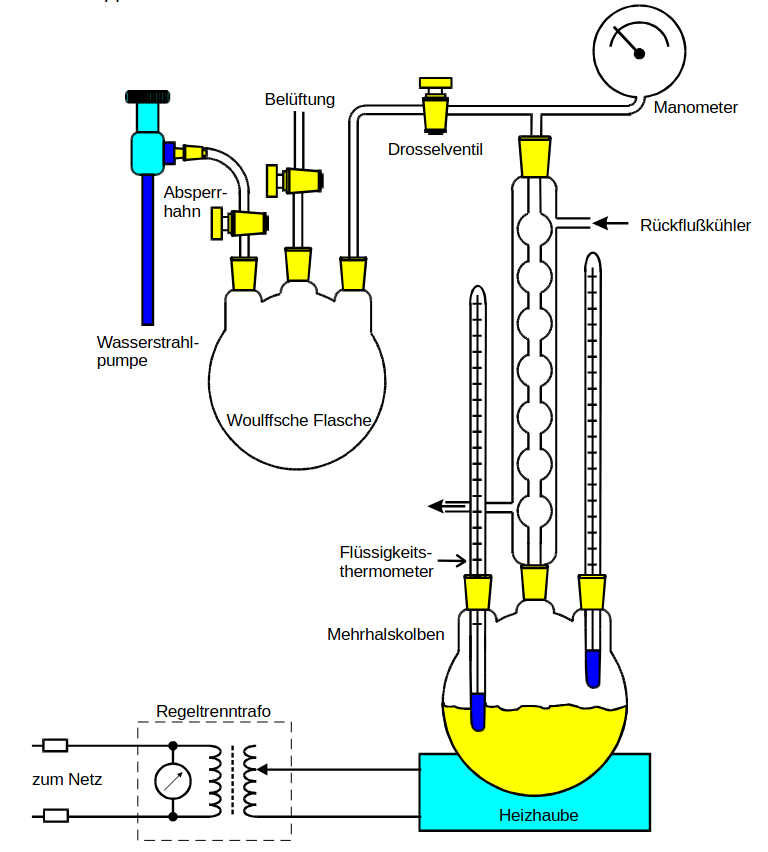
\includegraphics{"build/teil1.pdf"}
\end{figure}
Des weiteren Wurden die Werte aus \autoref{tab:10} in \autoref{fig:10} durch eine Funktion 
folgender Form geplottet.
\begin{equation}
    f\left(\phi\right) = a \cdot \sin \left(b \cdot \phi + c\right) + d
\end{equation}
Die ausgleichsrechnung mithilfe eines Curve Fits aus der Python Bibiliothek Scipy gibt 
die Ausgleichsparameter 
\begin{align*}
    a = & \qty{-6.1(0.4)}{\volt}   \\
    b = & \qty{1.00(0.04)}{}     \\
    c = & \qty{164(0.16)}{}    \\
    d = & \qty{0.00(0.31)}{\volt}      
\end{align*}
Die Parameter sind Für den Versuch uninteressant. Wichtiger ist der gut erkennbare 
sinusförmige Verlauf der Spannungsamplitude, der das eingangssignal wiedergibt. Die Parameter 
wären für einen vergleich interessant, sovern man die Messungen bei eingeschaltetem Rauschen 
noch einmal durchführen würde, was aucb der Hintergedanke dieses Experiemntes wäre, jedoch wird 
das nicht Durchgeführt, da die Geräte zu fehleranfällig sind.



%Intensität/Abstand
\begin{figure}[H]
    \caption{}
    \label{fig:11}
    \centering
    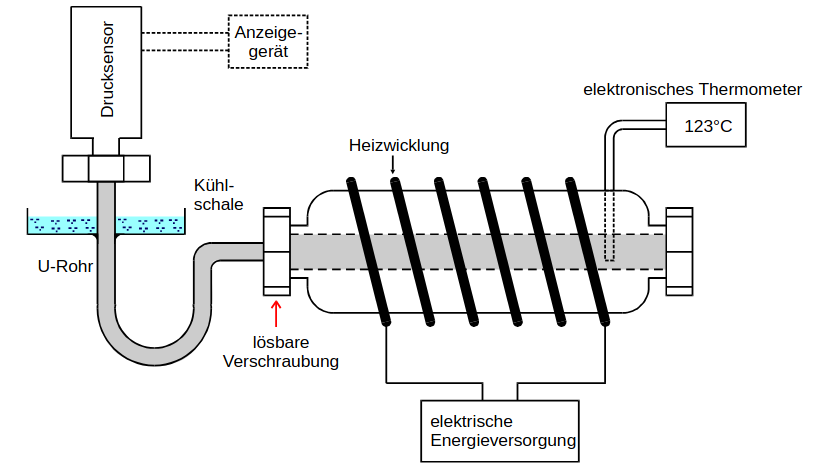
\includegraphics{"build/teil2.pdf"}
\end{figure}

\label{sec:Auswertung}
